\documentclass{standalone}
\usepackage{tikz}
\usepackage{ctex,siunitx}
\setCJKmainfont{Noto Serif CJK SC}
\usepackage{tkz-euclide}
\usepackage{amsmath}
\usetikzlibrary{patterns, calc,3d}
\usetikzlibrary {decorations.pathmorphing,decorations.pathreplacing,decorations.shapes}
\begin{document}
\small
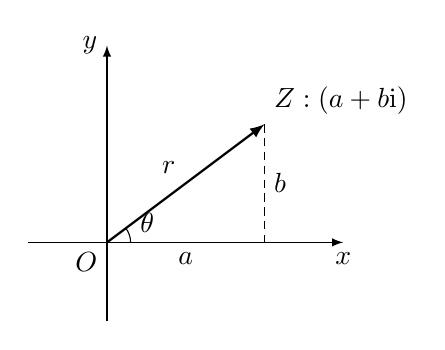
\begin{tikzpicture}[>=latex,scale=1.0]
  \draw[->](-1,0)--(3,0)node[below]{$x$};
  \draw[->](0,-1)--(0,2.5)node[left]{$y$};
  \node at (0,0)[below left]{$O$};
  \draw[thick,->](0,0)--(2,1.5)node[midway,above left]{$r$};
  \draw[densely dashed](2,1.5)--(2,0)node[midway,right]{$b$};
  \node at (2,1.5)[above right]{$Z:(a+b\mathrm{i})$};
  \node at (1,0)[below]{$a$};
  \draw(0.3,0)arc(0:37:0.3)node[at start,above right]{$\theta$};
\end{tikzpicture}
\end{document}